
\documentclass{article}
\usepackage[utf8]{inputenc}
\usepackage{amssymb}
\usepackage{tikz}
\usetikzlibrary{automata, positioning, arrows.meta}
\usepackage{enumitem}
\usepackage{subcaption}
\usepackage[fleqn]{amsmath}
\usepackage[top=2cm, bottom=2cm, left=2.5cm, right=2.5cm]{geometry}

\title{Automátas y Lenguajes Formales 25-2 \\ Tarea 4: Autómata mínimo y Teorema de Kleene}
\author{Hernández Vázquez Carlos Arturo }
\date{Martes 1 de Abril del 2025}

\begin{document}

\maketitle

\begin{enumerate}
    \item (3pts) Dado el siguiente autómata, convertirlo a un AFD y encontrar el autómata equivalente mînimo
        \begin{table}[h]
          \centering
          \begin{tabular}{c|c|c|c}
              $\delta$ & $a$ & $b$ & $\varepsilon$ \\ \hline
              *$\rightarrow q_0$ & $q_1$ & -- & -- \\
              $q_1$ & $q_4$ & $q_2$ & -- \\
              $q_2$ & $q_3$ & -- & $q_0$ \\
              $q_3$ & -- & $q_2$ & -- \\
              $q_4$ & -- & -- & $q_0$
          \end{tabular}
        \end{table}

        Como primer paso tenemos la $\epsilon$-cerradura de cada estado:
        \begin{table}[h]
          \centering
          \begin{tabular}{c|c}
              $\delta$ & $Cl_\varepsilon$ \\ \hline
              *$\rightarrow q_0$ & $\{q_0\}$ \\
              $q_1$ & $\{q_1\}$\\
              $q_2$ & $\{q_0, q_2\}$ \\
              $q_3$ & $\{q_3\}$ \\
              $q_4$ & $\{q_0, q_4\}$
          \end{tabular}
        \end{table}
        
        Hecho la anterior tenemos el AFN sin $\epsilon$-transiciones dado mediante $\delta$:
        \begin{align*}
        &\delta(q_0, a) = Cl_{\varepsilon}(\bigcup_{p \in Cl_{\varepsilon}(q_0)} \delta_{\varepsilon}(p,a)) = Cl_\varepsilon(\delta_\varepsilon(q_0,a)) = Cl_\varepsilon(\{q_1\}) = \{q_1\} \\
        &\delta(q_0, b) = Cl_{\varepsilon}(\bigcup_{p \in Cl_{\varepsilon}(q_0)} \delta_{\varepsilon}(p,b)) = Cl_\varepsilon(\delta_\varepsilon(q_0,b)) = Cl_\varepsilon (\varnothing) = \varnothing\\
        &\delta(q_1, a) = Cl_{\varepsilon}(\bigcup_{p \in Cl_{\varepsilon}(q_1)} \delta_{\varepsilon}(p,a)) = Cl_\varepsilon(\delta_\varepsilon(q_1,a)) = Cl_\varepsilon(\{q_4\}) = \{q_0, q_4\} \\
        &\delta(q_1, b) = Cl_{\varepsilon}(\bigcup_{p \in Cl_{\varepsilon}(q_1)} \delta_{\varepsilon}(p,b)) = Cl_\varepsilon(\delta_\varepsilon(q_1,b)) = Cl_\varepsilon(\{q_2\}) = \{q_0, q_2\} \\
        &\delta(q_2, a) = Cl_{\varepsilon}(\bigcup_{p \in Cl_{\varepsilon}(q_2)} \delta_{\varepsilon}(p,a)) = Cl_\varepsilon(\delta_\varepsilon(q_0,a) \cup \delta_\varepsilon(q_2, a)) = Cl_\varepsilon(\{q_1, q_3\}) = \{q_1, q_3\} \\
        &\delta(q_2, b) = Cl_{\varepsilon}(\bigcup_{p \in Cl_{\varepsilon}(q_2)} \delta_{\varepsilon}(p,b)) = Cl_\varepsilon(\delta_\varepsilon(q_0,b) \cup \delta_\varepsilon(q_2, b)) = Cl_\varepsilon(\ \varnothing ) = \varnothing\\
        &\delta(q_3, a) = Cl_{\varepsilon}(\bigcup_{p \in Cl_{\varepsilon}(q_3)} \delta_{\varepsilon}(p,a)) = Cl_\varepsilon(\delta_\varepsilon(q_3,a)) = Cl_\varepsilon(\varnothing) = \varnothing \\
        &\delta(q_3, b) = Cl_{\varepsilon}(\bigcup_{p \in Cl_{\varepsilon}(q_3)} \delta_{\varepsilon}(p,b)) = Cl_\varepsilon(\delta_\varepsilon(q_3,b)) = Cl_\varepsilon(\{q_2\}) = \{q_0, q_2\} \\
        &\delta(q_4, a) = Cl_{\varepsilon}(\bigcup_{p \in Cl_{\varepsilon}(q_4)} \delta_{\varepsilon}(p,a)) = Cl_\varepsilon(\delta_\varepsilon(q_0,a) \cup \delta_\varepsilon(q_4, a)) = Cl_\varepsilon(\{q_1\}) = \{q_1\} \\
        \end{align*}
        \begin{align*}
        &\delta(q_4, b) = Cl_{\varepsilon}(\bigcup_{p \in Cl_{\varepsilon}(q_4)} \delta_{\varepsilon}(p,b)) = Cl_\varepsilon(\delta_\varepsilon(q_0,b) \cup \delta_\varepsilon(q_4, b)) = Cl_\varepsilon(\varnothing) = \varnothing \\
        \end{align*}

        Para poder visualizar mejor cada transición se da la tabla del autómata:
        \begin{table}[h]
        \centering
          \begin{tabular}{c|c|c}
              $\delta$ & a & b \\
              \hline
              *$\rightarrow q_0$ & $q_1$ & $\varnothing$ \\
              $q_1$ & $q_0, q_4$ & $q_0, q_2$ \\
              $q_2$ & $q_1, q_3$ & $\varnothing$ \\
              $q_3$ & $\varnothing$ & $q_0, q_2$ \\
              $q_4$ & $q_1$ & $\varnothing$ \\
          \end{tabular}
        \end{table}

        Así, el AFD generado mediante la creación de conjuntos queda de la siguiente manera:
        \begin{table}[h]
            \centering
            \begin{tabular}{c c c c c}
                \begin{tabular}{c|c|c}
                    $\delta$ & a & b \\
                    \hline
                    *$\rightarrow q_0$ & $q_1$ & $\varnothing$ \\
                    $q_1$ & $q_0 q_4$ & $q_0 q_2$ \\
                    $*~ q_0 q_4$ & $q_1$ & $\varnothing$ \\
                    $*~ q_0 q_2$ & $q_1 q_3$ & $\varnothing$ \\
                    $q_1 q_3$ & $q_0 q_4$ & $q_0 q_2$ \\
                \end{tabular} 
                & 
                $\Longleftrightarrow$ 
                &
                \begin{tabular}{c|c|c}
                    $\delta$ & a & b \\
                    \hline
                    *$\rightarrow p_0$ & $p_1$ & $\varnothing$ \\
                    $p_1$ & $p_2$ & $p_3$ \\
                    $*~ p_2$ & $p_1$ & $\varnothing$ \\
                    $*~ p_3$ & $p_4$ & $\varnothing$ \\
                    $p_4$ & $p_2$ & $p_3$ \\
                \end{tabular}
            \end{tabular}
        \end{table}
    $$\text{(Se renombran los estados por claridad y comodidad)}$$

    Para el autómata minimo, primero notamos que por la forma en la que fue construido el AFD, todos los estados son alcanzables. Ahora, haciendo la distinción entre las estados finales y no finales:
    \begin{enumerate}
      \item Finales = $A = \{p_0, p_2, p_3\}$
      \item No finales = $B = \{p_1, p_4\}$
    \end{enumerate}
    Procediendo con las clases de equivalencia anteriores:
    \begin{table}[h]
      \centering
      \begin{tabular}{c | c | c | c | c | c}
        & \multicolumn{3}{c|}{A} & \multicolumn{2}{c}{B} \\    
        \hline
        & $p_0$ & $p_2$ & $p_3$ & $p_1$ & $p_4$  \\
        \hline
        a & B & B & B & A & A \\
        b & $\varnothing$ & $\varnothing$ & $\varnothing$ & A & A \\
      \end{tabular}
    \end{table}

    Debido a que no se formó una nueva clase de equivalencia, el autómata mínimo queda de la siguiente manera:
      \begin{table}[!h]
        \centering
          \begin{tabular}{c | c | c}
          & a & b \\
          \hline
            *$\rightarrow$ A & B & $\varnothing$ \\
            B & A & A \\
          \end{tabular}
      \end{table}

    \item (2.5pts) Minimiza el siguiente autómata y da una expresión regular utilizando el lema de Arden:
        \begin{table}[!h]
            \centering
            \begin{tabular}{c|c|c}
                $\delta$ & $a$ & $b$ \\ \hline
                $*~\rightarrow q_0$ & $q_1$ & $q_3$ \\
                $q_1$ & $q_2$ & $q_4$ \\
                * $q_2$ & $q_1$ & $q_5$ \\
                $q_3$ & $q_4$ & $q_0$ \\
                $q_4$ & $q_5$ & $q_1$ \\
                $q_5$ & $q_4$ & $q_2$
            \end{tabular}
        \end{table}
        \newline
        Primero podemos observar que no contiene estados inalcanzables, ya que de $q_0$ podemos llegar a $q_1$ y $q_3$; de $q_1$ a $q_2,q_4$; de $q_3$ a $q_4, q_0$; y de $q_4$ a $q_5, q_1$.\\

        \newpage
        Separamos los estados finales de los no finales:
        \begin{enumerate}
          \item Finales = $A = \{q_0, q_2\}$
          \item No finales = $B = \{q_1, q_3, q_4, q_5\}$
        \end{enumerate}
        \begin{table}[!h]
          \centering
          \begin{tabular}{c | c | c | c | c | c | c}
            & \multicolumn{2}{c|}{A} & \multicolumn{4}{c}{B} \\    
            \hline
            & $q_0$ & $q_2$ & $q_1$ & $q_3$ & $q_4$ & $q_5$   \\
            \hline
            a & B & B & A & B & B & B \\
            b & B & B & B & A & B & A
          \end{tabular}
        \end{table}

        Entonces obtenemos los siguiente grupos:
        \begin{enumerate}
          \item $A = \{q_0, q_2\}$
          \item $B = \{q_1\}$
          \item $C = \{q_3, q_5\}$
          \item $D = \{q_4\}$
        \end{enumerate}

        Partiendo de los anteriores se obtiene:
        \begin{table}[!h]
          \centering
          \begin{tabular}{c | c | c | c | c | c | c}
            & \multicolumn{2}{c|}{A} & \multicolumn{2}{c |}{C} & B & D \\    
            \hline
            & $q_0$ & $q_2$ & $q_3$ & $q_5$ & $q_1$ & $q_4$\\
            \hline
            a & B & B & D & D & A & C  \\
            b & C & C & A & A & D & B
          \end{tabular}
        \end{table}\\

        No se observan cambios, y por lo tanto el autómata minimo queda de la siguiente manera:
        \begin{table}[h]
          \centering
          \begin{tabular}{c | c | c}
          & a & b \\
          \hline
            *$\rightarrow$ A & B & C \\
            B & A & D \\
            C & D & A \\
            D & C & B
          \end{tabular}
        \end{table}

        Procediendo con la expresión regular. Analizando el autómata se consideran las siguientes ecuaciones:
        \begin{align}
          L(A) &= aL(B) + bL(C) + \varepsilon \\
          L(B) &= aL(A) + bL(D)\\
          L(C) &= aL(D) + bL(A)\\
          L(D) &= aL(C) + bL(B)
        \end{align}

        Sustituyendo $4$ en $2$
        \begin{equation}
        \begin{aligned}
          L(B) &= aL(A) + b(aL(C) + bL(B)) \\
               &= aL(A) + baL(C) + bbL(B) \\
               &= bbL(B) + aL(A) + baL(C) \\
               &= (bb)^* (aL(A) + baL(C)) \\
               &= (bb)^*aL(A) + (bb)^*baL(C)
        \end{aligned}
        \end{equation}

        Sustituyendo $4$ en $3$
        \begin{equation}
        \begin{aligned}
          L(C) &= a(aL(C) + bL(B)) + bL(A)\\
               &= aaL(C) + abL(B) + bL(A) 
        \end{aligned}
        \end{equation}

        Sustituyendo $5$ en $6$
        \begin{equation}
        \begin{aligned}
          L(C) &= aaL(C) + ab((bb)^*aL(A) + (bb)^*baL(C)) + bL(A)\\
                &= aaL(C) + ab(bb)^*aL(A) + ab(bb)^*baL(C) + bL(A) \\
                &= (aa + ab(bb)^*ba)L(C) + (b + ab(bb)^*a)L(A) \\
                &= (aa + ab(bb)^*ba)^* ((b + ab(bb)^*a)L(A))
        \end{aligned}
        \end{equation}
        Sustituyendo $5$ en $1$
        \begin{equation}
        \begin{aligned}
          L(A) &= a((bb)^*aL(A) + (bb)^*baL(C)) + bL(C) + \varepsilon \\
               &= a(bb)^*aL(A) + a(bb)^*baL(C) + bL(C) + \varepsilon \\
               &= a(bb)^*aL(A) + (a(bb)^*ba + b)L(C) + \varepsilon \\
        \end{aligned}
        \end{equation}
        Sustituyendo $7$ en $8$
        \begin{equation}
        \begin{aligned}
          L(A) &= a(bb)^*aL(A) + (a(bb)^*ba + b)((aa + ab(bb)^*ba)^* ((b + ab(bb)^*a)L(A))) + \varepsilon \\
               &= a(bb)^*aL(A) + (a(bb)^*ba + b)(aa + ab(bb)^*ba)^* ((b + ab(bb)^*a)L(A)) + \varepsilon \\
               &= (a(bb)^*a + (a(bb)^*ba + b)(aa + ab(bb)^*ba)^* ((b + ab(bb)^*a)))L(A) + \varepsilon \\
               &= (a(bb)^*a + (a(bb)^*ba + b)(aa + ab(bb)^*ba)^* ((b + ab(bb)^*a)))^*(\varepsilon)\\
               &= (a(bb)^*a + (a(bb)^*ba + b)(aa + ab(bb)^*ba)^* (b + ab(bb)^*a))^*\\
        \end{aligned}
        \end{equation}
        Entonces, la expresión regular para el autómata es
        $$\boxed{(a(bb)^*a + (a(bb)^*ba + b)(aa + ab(bb)^*ba)^* (b + ab(bb)^*a))^*}$$

    \item (1pt) Muestra un autómata finito que acepte el siguiente Lenguaje: $\alpha = (0 + 1)^* (01 + 110)$. Debes usar el Teorema de Kleene.\\
      Por un lado tenemos $0 + 1$:
        \begin{center}
            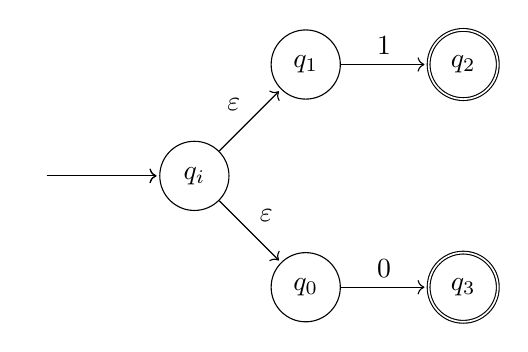
\begin{tikzpicture}[shorten >=1pt, node distance=2cm, on grid, auto]
                \tikzset{initial text={}}
                
                \node[state, initial] (qi) {$q_i$}; 
                \node[state] (q1) [above right=of qi] {$q_1$}; 
                \node[state] (q0) [below right=of qi] {$q_0$}; 

                \node[state, accepting] (q2) [right=of q1] {$q_2$};
                \node[state, accepting] (q3) [right=of q0] {$q_3$};

                \path[->]
                    (qi) edge node {$\varepsilon$} (q1)
                    (qi) edge node {$\varepsilon$} (q0)
                    (q1) edge node {1} (q2)
                    (q0) edge node {0} (q3);
                
                \node (start) [left=of qi] {};
                \draw[->] (start) -- (qi);

            \end{tikzpicture}
        \end{center}

        Aplicando * a la expresión anterior:
        \begin{center}
            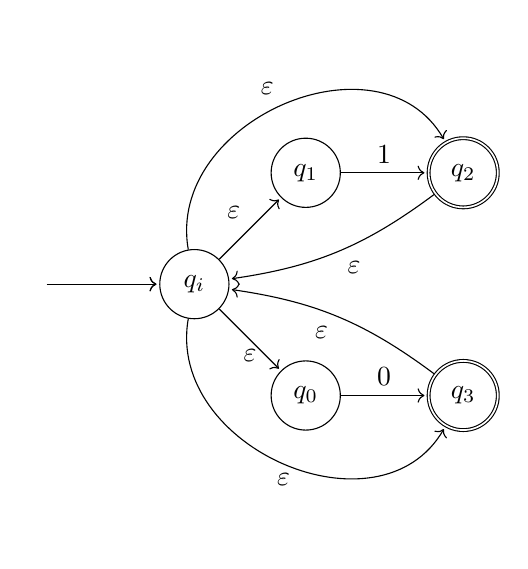
\begin{tikzpicture}[shorten >=1pt, node distance=2cm, on grid, auto]
                \tikzset{initial text={}}
                
                \node[state, initial] (qi) {$q_i$}; 
                \node[state] (q1) [above right=of qi] {$q_1$}; 
                \node[state] (q0) [below right=of qi] {$q_0$}; 

                \node[state, accepting] (q2) [right=of q1] {$q_2$};
                \node[state, accepting] (q3) [right=of q0] {$q_3$};

                \path[->]
                    (qi) edge node {$\varepsilon$} (q1)
                    (qi) edge node [below] {$\varepsilon$} (q0)
                    (qi) edge[out=100, in=120, looseness=1.2] node {$\varepsilon$} (q2)
                    (qi) edge[out=260, in=240, looseness=1.2] node [below] {$\varepsilon$} (q3)
                    (q1) edge node {1} (q2)
                    (q0) edge node {0} (q3)
                    (q3) edge [bend right=.5cm] node {$\varepsilon$} (qi)
                    (q2) edge [bend left=.5cm] node {$\varepsilon$} (qi);
                
                \node (start) [left=of qi] {};
                \draw[->] (start) -- (qi);

            \end{tikzpicture}
        \end{center}

        Por otro lado tenemos $01 + 110$:
        \begin{center}
            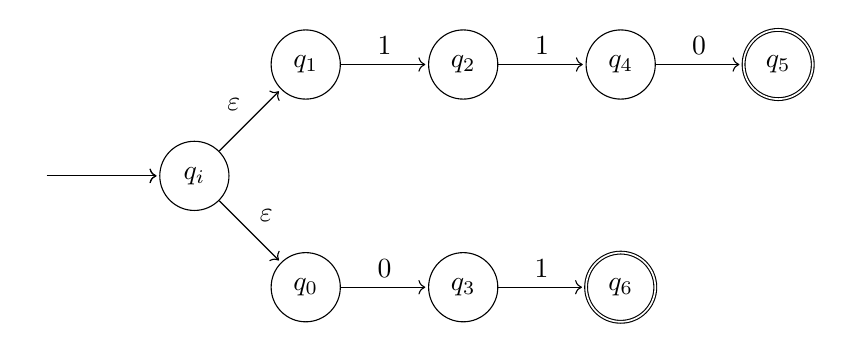
\begin{tikzpicture}[shorten >=1pt, node distance=2cm, on grid, auto]
                \tikzset{initial text={}}
                
                \node[state, initial] (qi) {$q_i$}; 
                \node[state] (q1) [above right=of qi] {$q_1$}; 
                \node[state] (q0) [below right=of qi] {$q_0$}; 

                \node[state] (q2) [right=of q1] {$q_2$};
                \node[state] (q4) [right=of q2] {$q_4$};
                \node[state, accepting] (q5) [right=of q4] {$q_5$};
                \node[state] (q3) [right=of q0] {$q_3$};
                \node[state, accepting] (q6) [right=of q3] {$q_6$};

                \path[->]
                    (qi) edge node {$\varepsilon$} (q1)
                    (qi) edge node {$\varepsilon$} (q0)
                    (q1) edge node {1} (q2)
                    (q2) edge node {1} (q4)
                    (q4) edge node {0} (q5)
                    (q3) edge node {1} (q6)
                    (q0) edge node {0} (q3);
                
                \node (start) [left=of qi] {};
                \draw[->] (start) -- (qi);

            \end{tikzpicture}
        \end{center}

        Concatenando los ultimos dos autómatas obtenemos el correspondiente para $(0 + 1)^*(01 + 110)$:

      \begin{center}
          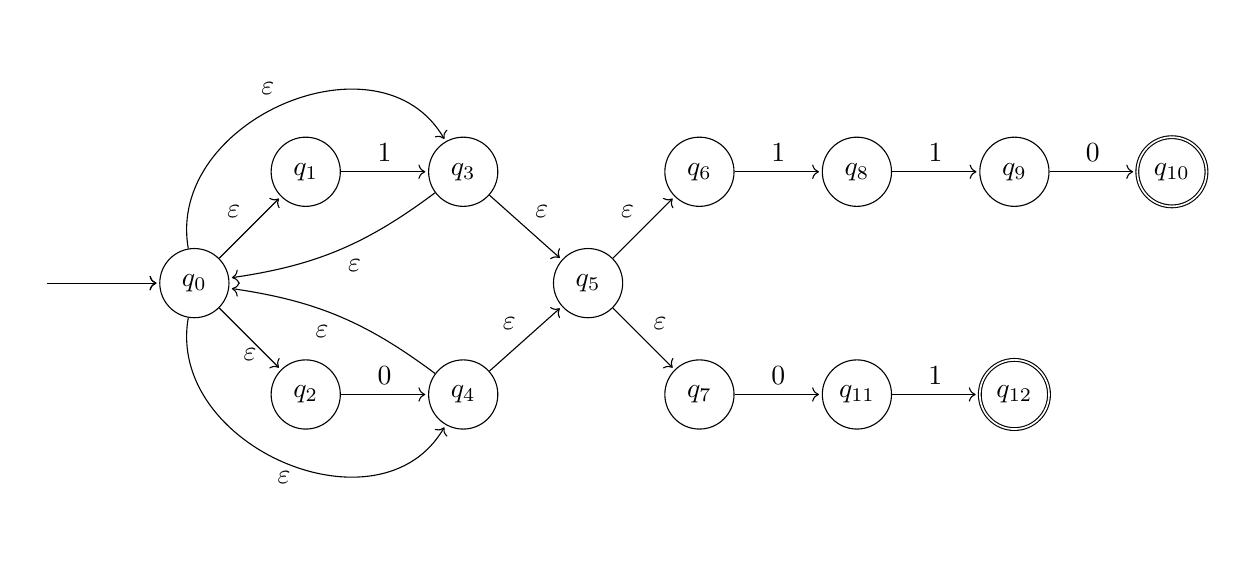
\begin{tikzpicture}[shorten >=1pt, node distance=2cm, on grid, auto]
              \tikzset{initial text={}}
              
              % Definición de nodos del primer autómata
              \node[state, initial] (q0) {$q_0$}; 
              \node[state] (q1) [above right=of q0] {$q_1$}; 
              \node[state] (q2) [below right=of q0] {$q_2$}; 
              \node[state] (q3) [right=of q1] {$q_3$};
              \node[state] (q4) [right=of q2] {$q_4$};

              % Transiciones del primer autómata
              \path[->]
                  (q0) edge node {$\varepsilon$} (q1)
                  (q0) edge node [below] {$\varepsilon$} (q2)
                  (q0) edge[out=100, in=120, looseness=1.2] node {$\varepsilon$} (q3)
                  (q0) edge[out=260, in=240, looseness=1.2] node [below] {$\varepsilon$} (q4)
                  (q1) edge node {1} (q3)
                  (q2) edge node {0} (q4)
                  (q4) edge [bend right=.5cm] node {$\varepsilon$} (q0)
                  (q3) edge [bend left=.5cm] node {$\varepsilon$} (q0);

              % Definición de nodos del segundo autómata con nombres cambiados
              \node[state] (q5) [right=5cm of q0] {$q_5$}; 
              \node[state] (q6) [above right=of q5] {$q_6$}; 
              \node[state] (q7) [below right=of q5] {$q_7$}; 
              \node[state] (q8) [right=of q6] {$q_8$};
              \node[state] (q9) [right=of q8] {$q_9$};
              \node[state, accepting] (q10) [right=of q9] {$q_{10}$};
              \node[state] (q11) [right=of q7] {$q_{11}$};
              \node[state, accepting] (q12) [right=of q11] {$q_{12}$};

              % Transiciones del segundo autómata
              \path[->]
                  (q5) edge node {$\varepsilon$} (q6)
                  (q5) edge node {$\varepsilon$} (q7)
                  (q6) edge node {1} (q8)
                  (q8) edge node {1} (q9)
                  (q9) edge node {0} (q10)
                  (q11) edge node {1} (q12)
                  (q7) edge node {0} (q11);

              % Conexión entre los autómatas
              \path[->]
                  (q3) edge node {$\varepsilon$} (q5)
                  (q4) edge node {$\varepsilon$} (q5);
              
              % Flecha de inicio
              \node (start) [left=of q0] {};
              \draw[->] (start) -- (q0);

          \end{tikzpicture}
      \end{center}

    \item (1.5pts) Minimiza el autómata del ejercicio anterior\\
      Como primer paso, sacamos la $\varepsilon$-cerradura de cada estado:
      \begin{table}[h]
        \centering
          \begin{tabular}{c|c}
               & $Cl_\varepsilon$ \\ \hline
              $q_0$ & $q_0,q_1,q_2,q_3,q_4,q_5,q_6,q_7$  \\
              $q_1$ & $q_1$  \\
              $q_2$ & $q_2$  \\
              $q_3$ & $q_0,q_1,q_2,q_3,q_4,q_5,q_6,q_7$  \\
              $q_4$ & $q_0,q_1,q_2,q_3,q_4,q_5,q_6,q_7$  \\
              $q_5$ & $q_5,q_6,q_7$  \\
              $q_6$ & $q_6$  \\
              $q_7$ & $q_7$  \\
              $q_8$ & $q_8$  \\
              $q_9$ & $q_9$  \\
              $q_{10}$ & $q_{10}$  \\
              $q_{11}$ & $q_{11}$  \\
              $q_{12}$ & $q_{12}$  \\
          \end{tabular}
      \end{table}

      Asi, el AFN sin $\varepsilon$-transiciones queda definido por las siguiente transiciones:
      \begin{align*}
        \delta(q_0, 0) &= Cl_{\varepsilon}(\bigcup_{p \in Cl_{\varepsilon}(q_0)} \delta_{\varepsilon}(p,0)) \\
          &= Cl_\varepsilon(\delta_\varepsilon(q_0,0) \cup \delta_\varepsilon(q_1,0) \cup \delta_\varepsilon(q_2, 0) \cup \delta_\varepsilon(q_3, 0) \cup \delta_\varepsilon(q_4, 0) \cup \delta_\varepsilon(q_5,0) \cup \delta_\varepsilon(q_6, 0) \cup \delta_\varepsilon(q_7,0)) \\
          &= Cl_\varepsilon(\{q_4,q_{11}\}) = \{q_0,q_1,q_2,q_3,q_4,q_5,q_6,q_7,q_{11}\}\\
      \end{align*}
      \begin{align*}
        \delta(q_0, 1) &= Cl_{\varepsilon}(\bigcup_{p \in Cl_{\varepsilon}(q_0)} \delta_{\varepsilon}(p,1)) \\
          &= Cl_\varepsilon(\delta_\varepsilon(q_0,1) \cup \delta_\varepsilon(q_1,1) \cup \delta_\varepsilon(q_2, 1) \cup \delta_\varepsilon(q_3,1) \cup \delta_\varepsilon(q_4, 1) \cup \delta_\varepsilon(q_5,1) \cup \delta_\varepsilon(q_6, 1) \cup \delta_\varepsilon(q_7,1)) \\
          &= Cl_\varepsilon(\{q_3,q_8\}) = \{q_0,q_1,q_2,q_3,q_4,q_5,q_6,q_7,q_8\}\\
      \end{align*}
      \begin{align*}
        \delta(q_1, 0) &= Cl_{\varepsilon}(\bigcup_{p \in Cl_{\varepsilon}(q_1)} \delta_{\varepsilon}(p,0)) = Cl_\varepsilon(\delta_\varepsilon(q_1,0)) = Cl_\varepsilon(\varnothing) = \varnothing
      \end{align*}
      \begin{align*}
        \delta(q_1, 1) &= Cl_{\varepsilon}(\bigcup_{p \in Cl_{\varepsilon}(q_1)} \delta_{\varepsilon}(p,1)) = Cl_\varepsilon(\delta_\varepsilon(q_1,1)) = Cl_\varepsilon(\{q_3\}) = \{q_0,q_1,q_2,q_3,q_4,q_5,q_6,q_7\}
      \end{align*}
      \begin{align*}
      \delta(q_2, 0) &= Cl_{\varepsilon}(\bigcup_{p \in Cl_{\varepsilon}(q_2)} \delta_{\varepsilon}(p,0)) = Cl_\varepsilon(\delta_\varepsilon(q_2,0)) = Cl_\varepsilon(\{q_4\}) = \{q_0,q_1,q_2,q_3,q_4,q_5,q_6,q_7\} \\
      \end{align*}
      \begin{align*}
      \delta(q_2, 1) &= Cl_{\varepsilon}(\bigcup_{p \in Cl_{\varepsilon}(q_2)} \delta_{\varepsilon}(p,1)) = Cl_\varepsilon(\delta_\varepsilon(q_2,1)) = Cl_\varepsilon(\varnothing) = \varnothing \\
      \end{align*}
      \begin{align*}
        \delta(q_3, 0) &= Cl_{\varepsilon}(\bigcup_{p \in Cl_{\varepsilon}(q_3)} \delta_{\varepsilon}(p,0)) \\
          &= Cl_\varepsilon(\delta_\varepsilon(q_0,0) \cup \delta_\varepsilon(q_1,0) \cup \delta_\varepsilon(q_2, 0) \cup \delta_\varepsilon(q_3, 0) \cup \delta_\varepsilon(q_4, 0) \cup \delta_\varepsilon(q_5,0) \cup \delta_\varepsilon(q_6, 0) \cup \delta_\varepsilon(q_7,0)) \\
          &= Cl_\varepsilon(\{q_4,q_{11}\}) = \{q_0,q_1,q_2,q_3,q_4,q_5,q_6,q_7,q_{11}\}\\
      \end{align*}
      \begin{align*}
        \delta(q_3, 1) &= Cl_{\varepsilon}(\bigcup_{p \in Cl_{\varepsilon}(q_3)} \delta_{\varepsilon}(p,1)) \\
          &= Cl_\varepsilon(\delta_\varepsilon(q_0,1) \cup \delta_\varepsilon(q_1,1) \cup \delta_\varepsilon(q_2, 1) \cup \delta_\varepsilon(q_3,1) \cup \delta_\varepsilon(q_4, 1) \cup \delta_\varepsilon(q_5,1) \cup \delta_\varepsilon(q_6, 1) \cup \delta_\varepsilon(q_7,1)) \\
          &= Cl_\varepsilon(\{q_3,q_8\}) = \{q_0,q_1,q_2,q_3,q_4,q_5,q_6,q_7,q_8\}\\
      \end{align*}
      \begin{align*}
        \delta(q_4, 0) &= Cl_{\varepsilon}(\bigcup_{p \in Cl_{\varepsilon}(q_4)} \delta_{\varepsilon}(p,0)) \\
          &= Cl_\varepsilon(\delta_\varepsilon(q_0,0) \cup \delta_\varepsilon(q_1,0) \cup \delta_\varepsilon(q_2, 0) \cup \delta_\varepsilon(q_3, 0) \cup \delta_\varepsilon(q_4, 0) \cup \delta_\varepsilon(q_5,0) \cup \delta_\varepsilon(q_6, 0) \cup \delta_\varepsilon(q_7,0)) \\
          &= Cl_\varepsilon(\{q_4,q_{11}\}) = \{q_0,q_1,q_2,q_3,q_4,q_5,q_6,q_7,q_{11}\}\\
      \end{align*}
      \begin{align*}
        \delta(q_4, 1) &= Cl_{\varepsilon}(\bigcup_{p \in Cl_{\varepsilon}(q_4)} \delta_{\varepsilon}(p,1)) \\
          &= Cl_\varepsilon(\delta_\varepsilon(q_0,1) \cup \delta_\varepsilon(q_1,1) \cup \delta_\varepsilon(q_2, 1) \cup \delta_\varepsilon(q_3,1) \cup \delta_\varepsilon(q_4, 1) \cup \delta_\varepsilon(q_5,1) \cup \delta_\varepsilon(q_6, 1) \cup \delta_\varepsilon(q_7,1)) \\
          &= Cl_\varepsilon(\{q_3,q_8\}) = \{q_0,q_1,q_2,q_3,q_4,q_5,q_6,q_7,q_8\}\\
      \end{align*}
      \begin{align*}
        \delta(q_5, 0) &= Cl_{\varepsilon}(\bigcup_{p \in Cl_{\varepsilon}(q_5)} \delta_{\varepsilon}(p,0)) = Cl_\varepsilon(\delta_\varepsilon(q_5,0) \cup \delta_\varepsilon(q_6,0) \cup \delta_\varepsilon(q_7, 0)) = Cl_\varepsilon(\{q_{11}\}) = \{q_{11}\}\\
      \end{align*}
      \begin{align*}
        \delta(q_5, 1) &= Cl_{\varepsilon}(\bigcup_{p \in Cl_{\varepsilon}(q_5)} \delta_{\varepsilon}(p,1)) = Cl_\varepsilon(\delta_\varepsilon(q_5,1) \cup \delta_\varepsilon(q_6,1) \cup \delta_\varepsilon(q_7,1)) = Cl_\varepsilon(\{q_8\}) = \{q_8\}\\
      \end{align*}
      \begin{align*}
        \delta(q_6, 0) &= Cl_{\varepsilon}(\bigcup_{p \in Cl_{\varepsilon}(q_6)} \delta_{\varepsilon}(p,0)) = Cl_\varepsilon(\delta_\varepsilon(q_6,0)) = Cl_\varepsilon(\varnothing) = \varnothing\\ 
      \end{align*}
      \begin{align*}
        \delta(q_6, 1) &= Cl_{\varepsilon}(\bigcup_{p \in Cl_{\varepsilon}(q_6)} \delta_{\varepsilon}(p,1)) = Cl_\varepsilon(\delta_\varepsilon(q_6,1)) = Cl_\varepsilon(\{q_8\}) = \{q_8\}\\
      \end{align*}
      \begin{align*}
        \delta(q_7, 0) &= Cl_{\varepsilon}(\bigcup_{p \in Cl_{\varepsilon}(q_7)} \delta_{\varepsilon}(p,0)) = Cl_\varepsilon(\delta_\varepsilon(q_7,0)) = Cl_\varepsilon(\{q_{11}\}) = \{q_{11}\}\\
      \end{align*}
      \begin{align*}
        \delta(q_7, 1) &= Cl_{\varepsilon}(\bigcup_{p \in Cl_{\varepsilon}(q_7)} \delta_{\varepsilon}(p,1)) = Cl_\varepsilon(\delta_\varepsilon(q_7,1)) = Cl_\varepsilon(\varnothing) = \varnothing\\
      \end{align*}
      \begin{align*}
        \delta(q_8, 0) &= Cl_{\varepsilon}(\bigcup_{p \in Cl_{\varepsilon}(q_8)} \delta_{\varepsilon}(p,0)) = Cl_\varepsilon(\delta_\varepsilon(q_8,0)) = Cl_\varepsilon(\varnothing) = \varnothing\\
      \end{align*}
      \begin{align*}
        \delta(q_8, 1) &= Cl_{\varepsilon}(\bigcup_{p \in Cl_{\varepsilon}(q_8)} \delta_{\varepsilon}(p,1)) = Cl_\varepsilon(\delta_\varepsilon(q_8,1)) = Cl_\varepsilon(\{q_9\}) = \{q_9\}\\
      \end{align*}
      \begin{align*}
        \delta(q_9, 0) &= Cl_{\varepsilon}(\bigcup_{p \in Cl_{\varepsilon}(q_9)} \delta_{\varepsilon}(p,0)) = Cl_\varepsilon(\delta_\varepsilon(q_9,0)) = Cl_\varepsilon(\{q_{10}\}) = \{q_{10}\}\\
      \end{align*}
      \begin{align*}
        \delta(q_9, 1) &= Cl_{\varepsilon}(\bigcup_{p \in Cl_{\varepsilon}(q_9)} \delta_{\varepsilon}(p,1)) = Cl_\varepsilon(\delta_\varepsilon(q_9,1)) = Cl_\varepsilon(\varnothing) = \varnothing\\
      \end{align*}
      \begin{align*}
        \delta(q_{10}, 0) &= Cl_{\varepsilon}(\bigcup_{p \in Cl_{\varepsilon}(q_{10})} \delta_{\varepsilon}(p,0)) = Cl_\varepsilon(\delta_\varepsilon(q_{10},0)) = Cl_\varepsilon(\varnothing) = \varnothing\\
      \end{align*}
      \begin{align*}
        \delta(q_{10}, 1) &= Cl_{\varepsilon}(\bigcup_{p \in Cl_{\varepsilon}(q_{10})} \delta_{\varepsilon}(p,1)) = Cl_\varepsilon(\delta_\varepsilon(q_{10},1)) = Cl_\varepsilon(\varnothing) = \varnothing\\
      \end{align*}
      \begin{align*}
        \delta(q_{11}, 0) &= Cl_{\varepsilon}(\bigcup_{p \in Cl_{\varepsilon}(q_{11})} \delta_{\varepsilon}(p,0)) = Cl_\varepsilon(\delta_\varepsilon(q_{11},0)) = Cl_\varepsilon(\varnothing) = \varnothing\\
      \end{align*}
      \begin{align*}
        \delta(q_{11}, 1) &= Cl_{\varepsilon}(\bigcup_{p \in Cl_{\varepsilon}(q_{11})} \delta_{\varepsilon}(p,1)) = Cl_\varepsilon(\delta_\varepsilon(q_{11},1)) = Cl_\varepsilon(\{q_{12}\}) = \{q_{12}\}\\
      \end{align*}
      \begin{align*}
        \delta(q_{12}, 0) &= Cl_{\varepsilon}(\bigcup_{p \in Cl_{\varepsilon}(q_{12})} \delta_{\varepsilon}(p,0)) = Cl_\varepsilon(\delta_\varepsilon(q_{12},0)) = Cl_\varepsilon(\varnothing) = \varnothing\\
      \end{align*}
      \begin{align*}
        \delta(q_{12}, 1) &= Cl_{\varepsilon}(\bigcup_{p \in Cl_{\varepsilon}(q_{12})} \delta_{\varepsilon}(p,1)) = Cl_\varepsilon(\delta_\varepsilon(q_{12},1)) = Cl_\varepsilon(\varnothing) = \varnothing\\
      \end{align*}

      Usando lo anterior, el AFD queda de la siguiente manera:
    \begin{table}[!h]
      \centering
        \begin{tabular}{c|c|c}
            $\delta$ & $0$ & $1$ \\ \hline
            $\rightarrow q_0$ & $q_0q_1q_2q_3q_4q_5q_6q_7q_{11}$ & $q_0q_1q_2q_3q_4q_5q_6q_7q_8$ \\
            $q_0q_1q_2q_3q_4q_5q_6q_7q_{11}$ & $q_0q_1q_2q_3q_4q_5q_6q_7q_{11}$& $q_0q_1q_2q_3q_4q_5q_6q_7q_8q_{12}$\\
            $q_0q_1q_2q_3q_4q_5q_6q_7q_8$ & $q_0q_1q_2q_3q_4q_5q_6q_7q_{11}$& $q_0q_1q_2q_3q_4q_5q_6q_7q_8q_9$\\
            *$q_0q_1q_2q_3q_4q_5q_6q_7q_8q_{12}$ & $q_0q_1q_2q_3q_4q_5q_6q_7q_{11}$ & $q_0q_1q_2q_3q_4q_5q_6q_7q_8q_9$\\
            $q_0q_1q_2q_3q_4q_5q_6q_7q_8q_9$ & $q_0q_1q_2q_3q_4q_5q_6q_7q_{10}q_{11}$& $q_0q_1q_2q_3q_4q_5q_6q_7q_8q_9$ \\
            *$q_0q_1q_2q_3q_4q_5q_6q_7q_{10}q_{11}$ & $q_0q_1q_2q_3q_4q_5q_6q_7q_{11}$& $q_0q_1q_2q_3q_4q_5q_6q_7q_8q_{12}$
        \end{tabular}
    \end{table}\\

    Renombrando los estados:
    \begin{table}[!h]
      \centering
        \begin{tabular}{c|c|c}
            $\delta$ & $0$ & $1$ \\ \hline
            $\rightarrow p_0$ & $p_1$ & $p_2$ \\
            $p_1$ & $p_1$ & $p_3$\\
            $p_2$ & $p_1$ & $p_4$\\
            *$p_3$ & $p_1$ & $p_4$\\
            $p_4$ & $p_5$ & $p_4$ \\
            *$p_5$ & $p_1$ & $p_3$ 
        \end{tabular}

    \end{table}\\
        Comenzando a minimizar. Por la construcción del AFD, todos los estados son alcanzables. Asi que se procede separando los estados finales y los no finales:
        \begin{enumerate}
          \item Finales = $A = \{p_3, p_5\}$
          \item No finales = $B = \{p_0, p_1, p_2, p_4\}$
        \end{enumerate}

        Con ello, comienza la primera etapa:
        \begin{table}[!h]
          \centering
          \begin{tabular}{c | c | c | c | c | c | c}
            & \multicolumn{2}{c|}{A} & \multicolumn{4}{c}{B} \\    
            \hline
            & $p_3$ & $p_5$ & $p_0$ & $p_1$ & $p_2$ & $p_4$   \\
            \hline
            0 & B & B & B & B & B & A  \\
            1 & B & A & B & A & B & B
          \end{tabular}
        \end{table}
        \newpage
        Entonces obtenemos los siguiente grupos:
        \begin{enumerate}
          \item $A = \{p_3\}$
          \item $B = \{p_5\}$
          \item $C = \{p_0, p_2\}$
          \item $D = \{p_1\}$
          \item $E = \{p_4\}$
        \end{enumerate}

        Continuamos con las clases de equivalencia obtenidas:
        \begin{table}[!h]
          \centering
          \begin{tabular}{c | c | c | c | c | c | c}
            & \multicolumn{1}{c|}{A} & \multicolumn{1}{c|}{B} & \multicolumn{2}{c|}{C} & D & E \\    
            \hline
            & $p_3$ & $p_5$ & $p_0$ & $p_2$ & $p_1$ & $p_4$   \\
            \hline
            0 & D & D & D & D & D & B \\
            1 & E & A & C & E & A & E
          \end{tabular}
        \end{table}
        
        Observando la tabla, se puede apreciar que cada estado original quedó separando de los demás. Es decir, el AFD obtenido en primera instancia ya era el mínimo. El diagrama correspondiente queda de la siguiente forma:

        \begin{center}
            \begin{tikzpicture}[shorten >=1pt, node distance=2cm, on grid, auto]
                \tikzset{initial text={}}
                
                \node[state, initial] (p0) {$p_0$}; 
                \node[state] (p1) [right=of p0] {$p_1$}; 
                \node[state] (p2) [below =of p0] {$p_2$}; 
                \node[state, accepting] (p3) [right=of p1] {$p_3$}; 
                \node[state] (p4) [right=of p2] {$p_4$}; 
                \node[state, accepting] (p5) [right=of p4] {$p_5$}; 

                \path[->]
                    (p0) edge node {0} (p1)
                    (p0) edge node [left] {1} (p2)
                    (p1) edge [loop above] node {0} (p1)
                    (p1) edge [bend left] node {1} (p3)
                    (p2) edge node {0} (p1)
                    (p2) edge node [below] {1} (p4)
                    (p3) edge node {0} (p1)
                    (p3) edge node [near end, left] {1} (p4)
                    (p4) edge [loop below] node {1} (p4)
                    (p4) edge node [below] {0} (p5)
                    (p5) edge node [right] {1} (p3)
                    (p5) edge node [near start] {0} (p1);
                
                \node (start) [left=of qi] {};
                \draw[->] (start) -- (qi);

            \end{tikzpicture}
        \end{center}

    \item (3pts) utilizando el Lema de Arden, calcula una expresión regular para cada una de los siguientes autómatas, muestra las ecuaciones y los pasos para obtener la expresión.

    \underline{Primer autómata}
    \begin{table}[h]
      \centering
        \begin{tabular}{c|c|c}
            $\delta$ & $a$ & $b$ \\ \hline
            $\rightarrow q_0$ & $q_1$ & $q_3$ \\
            * $q_1$ & -- & $q_2$ \\
            $q_2$ & $q_1$ & $q_2$ \\
            $q_3$ & $q_1$ & --
        \end{tabular}
    \end{table}

    \setcounter{equation}{0}
    De la tabla anterior tenemos las siguiente ecuaciones:
    \begin{align}
      L(q_0) &= aL(q_1) + bL(q_3) \\
      L(q_1) &= bL(q_2) + \varepsilon \\
      L(q_2) &= aL(q_1) + bL(q_2) \\
      L(q_3) &= aL(q_1) 
    \end{align}

    De $3$ obtenemos
    \begin{align}
      L(q_2) = aL(q_1) + bL(q_2) = b^*(aL(q_1))
    \end{align}

    Sustituyendo $5$ en $2$
    \begin{align}
      L(q_1) &= bb^*aL(q_1) + \varepsilon = (bb^*a)^*\varepsilon = (bb^*a)^*
    \end{align}

    Sustituyendo $6$ en $4$
    \begin{align}
      L(q_3) &= a(bb^*a)^*
    \end{align}

    Por $6, 7$ en $1$
    \begin{align}
      L(q_0) &= a(bb^*a)^* + ba(bb^*a)^* = (a + ba)(bb^*a)^*
    \end{align}

    Entonces, la expresión regular para el autómata dado es
    $$\boxed{a(bb^*a)^* + ba(bb^*a)^* = (a + ba)(bb^*a)^*}$$

    \underline{Segundo autómata:}
    \begin{table}[h]
      \centering
        \begin{tabular}{c|c|c}
            $\delta$ & $a$ & $b$ \\ \hline
            *$\rightarrow q_0$ & $q_0$ & $q_1$ \\
          * $q_1$ & $q_2$ & $q_1$ \\
          * $q_2$ & $q_0$ & $q_3$ \\
          * $q_3$ & $q_3$ & $q_3$
        \end{tabular}
    \end{table}\\

    \setcounter{equation}{0}
    Tenemos las siguiente ecuaciones
    \begin{align}
      L(q_0) &= aL(q_0) + bL(q_1) + \varepsilon \\
      L(q_1) &= aL(q_2) + bL(q_1) + \varepsilon \\
      L(q_2) &= aL(q_0) + bL(q_3) + \varepsilon \\
      L(q_3) &= aL(q_3) + bL(q_3) + \varepsilon 
    \end{align}
    \end{enumerate}

    De $3$ obtenemos
    \begin{equation}
    \begin{aligned}
      L(q_3) &= (a + b)L(q_3) + \varepsilon \\
            &= (a + b)^* (\varepsilon) \\
            &= (a + b)^* 
    \end{aligned}
    \end{equation}

    Sustituyendo $5$ en $3$
    \begin{equation}
    \begin{aligned}
      L(q_2) &= aL(q_0) + b(a+b)^* + \varepsilon \\
    \end{aligned}
    \end{equation}

    Sustituyendo $6$ en $2$
    \begin{equation}
    \begin{aligned}
      L(q_1) &= a(aL(q_0) + b(a+b)^* + \varepsilon) + bL(q_1) + \varepsilon \\
            &= aaL(q_0) + ab(a+b)^* + a + bL(q_1) + \varepsilon \\
            &= b^* (aaL(q_0) + ab(a+b)^* + a + \varepsilon )\\
            &= b^*aaL(q_0) + b^*ab(a+b)^* + b^*a + b^* \\
    \end{aligned}
    \end{equation}

    Sustituyendo $7$ en $1$
    \begin{equation}
    \begin{aligned}
      L(q_0) &= aL(q_0) + b(b^*aaL(q_0) + b^*ab(a+b)^* + b^*a + b^* ) + \varepsilon \\
            &= aL(q_0) + bb^*aaL(q_0) + bb^*ab(a+b)^* + bb^*a + bb^* + \varepsilon \\
            &= (a + bb^*aa)L(q_0) + bb^*ab(a+b)^* + bb^*a + bb^* + \varepsilon \\
            &= (a + bb^*aa)^* (bb^*ab(a+b)^* + bb^*a + bb^* + \varepsilon)\\
            &= (a + b^+aa)^* (b^+ab(a+b)^* + b^+a + b^+ + \varepsilon)\\
    \end{aligned}
    \end{equation}

    Entonces, la expresión regular para el autómata es 
    $$\boxed{(a + b^+aa)^* (b^+ab(a+b)^* + b^+a + b^+ + \varepsilon)}$$


\end{document}
